\documentclass[10pt,openany]{book}
\usepackage[utf8]{inputenc}
\DeclareUnicodeCharacter{2212}{\ensuremath{-}}
\DeclareUnicodeCharacter{2192}{\ensuremath{\to}}
\DeclareUnicodeCharacter{03B1}{\ensuremath{\alpha}}
\usepackage[T1]{fontenc}
\usepackage{lmodern}
\usepackage[spanish,es-nodecimaldot]{babel}
\spanishplainpercent
\AtBeginDocument{\spanishdeactivate{"~<>}}
\usepackage[a4paper,margin=2.5cm,headheight=14pt]{geometry}
\usepackage{amsmath,amssymb,mathtools,booktabs,array,longtable,graphicx,xcolor,tikz,enumitem,microtype,titlesec,fancyhdr}
\usepackage[breakable,skins]{tcolorbox}
\usepackage[labelfont=bf]{caption}
\usepackage[hyphens]{url}
\usepackage[hidelinks,unicode,hypertexnames=false]{hyperref}
\definecolor{studiumInk}{RGB}{20,44,64}
\definecolor{studiumBlue}{RGB}{24,74,130}
\definecolor{studiumCyan}{RGB}{0,184,205}
\definecolor{studiumLight}{RGB}{232,240,250}
\definecolor{studiumWorkedBack}{RGB}{255,244,230}
\definecolor{studiumWorkedFrame}{RGB}{138,78,12}
\definecolor{studiumCheckBack}{RGB}{243,236,248}
\definecolor{studiumCheckFrame}{RGB}{96,48,130}
\titleformat{\chapter}[display]{\normalfont\filright}{\large\scshape\chaptertitlename\ \thechapter}{1ex}{\huge\bfseries}
\titlespacing*{\chapter}{0pt}{2.5ex plus 1ex minus .2ex}{2.3ex}
\titleformat{name=\chapter,numberless}[display]{\normalfont\filright}{}{0pt}{\huge\bfseries}
\titleformat{\section}{\Large\bfseries}{\thesection}{.8em}{}
\titleformat{\subsection}{\large\bfseries}{\thesubsection}{.7em}{}
\makeatletter
\renewcommand*\l@section{\@dottedtocline{1}{1.5em}{3.5em}}
\makeatother
\setcounter{secnumdepth}{2}\setcounter{tocdepth}{1}
\setlength{\parindent}{1.5em}\setlength{\parskip}{3pt plus .5pt}
\setlength{\emergencystretch}{1.5em}\raggedbottom
\setlist{itemsep=2pt,topsep=4pt,leftmargin=*}
\allowdisplaybreaks[2]
\graphicspath{{../figures/}}
\newcommand{\Raire}{287.05287}
\newcommand{\gzero}{9.80665}
\tcbset{studiumcommon/.style={breakable,boxrule=.65pt,arc=.7pt,left=1.7mm,right=1.7mm,top=1.3mm,bottom=1.3mm,before skip=10pt,after skip=10pt,fonttitle=\bfseries}}
\newtcolorbox{studiumworked}[1]{studiumcommon,colback=studiumWorkedBack,colframe=studiumWorkedFrame,colbacktitle=studiumWorkedFrame,coltitle=white,title={#1}}
\newcommand{\objetivos}[1]{\par\noindent\textbf{Objetivos de aprendizaje.} \textit{#1}\par\medskip}
\newcommand{\caja}[2]{\begin{tcolorbox}[studiumcommon,colback=studiumLight,colframe=studiumBlue,colbacktitle=studiumBlue,coltitle=white,title={#1}]#2\end{tcolorbox}}
\newcommand{\resumen}[1]{\begin{tcolorbox}[studiumcommon,colback=studiumCheckBack,colframe=studiumCheckFrame,colbacktitle=studiumCheckFrame,coltitle=white,title=Resumen]#1\end{tcolorbox}}
\newcommand{\figura}[2]{\begin{figure}[tbp]\centering\includegraphics[width=.83\linewidth]{#1.pdf}\caption{#2}\label{fig:#1}\end{figure}\noindent La figura~\ref{fig:#1} ofrece una representación del modelo discutido.}
\pagestyle{fancy}\fancyhf{}
\fancyhead[LE]{\small\thepage\hspace{1.5em}\scshape\nouppercase{\leftmark}}
\fancyhead[RO]{\small\scshape\nouppercase{\rightmark}\hspace{1.5em}\thepage}
\renewcommand{\headrulewidth}{.4pt}\renewcommand{\footrulewidth}{0pt}
\fancypagestyle{plain}{\fancyhf{}\fancyfoot[C]{\small\thepage}\renewcommand{\headrulewidth}{0pt}}
\newcommand{\portada}[2]{\hypersetup{pageanchor=false}\begin{titlepage}\thispagestyle{empty}
\begin{tikzpicture}[remember picture,overlay,x=1pt,y=-1pt]
\begin{scope}[shift={(current page.north west)}]
\clip (0,0) rectangle (595.276,841.89);
\node[inner sep=0pt] at (297.638,420.945){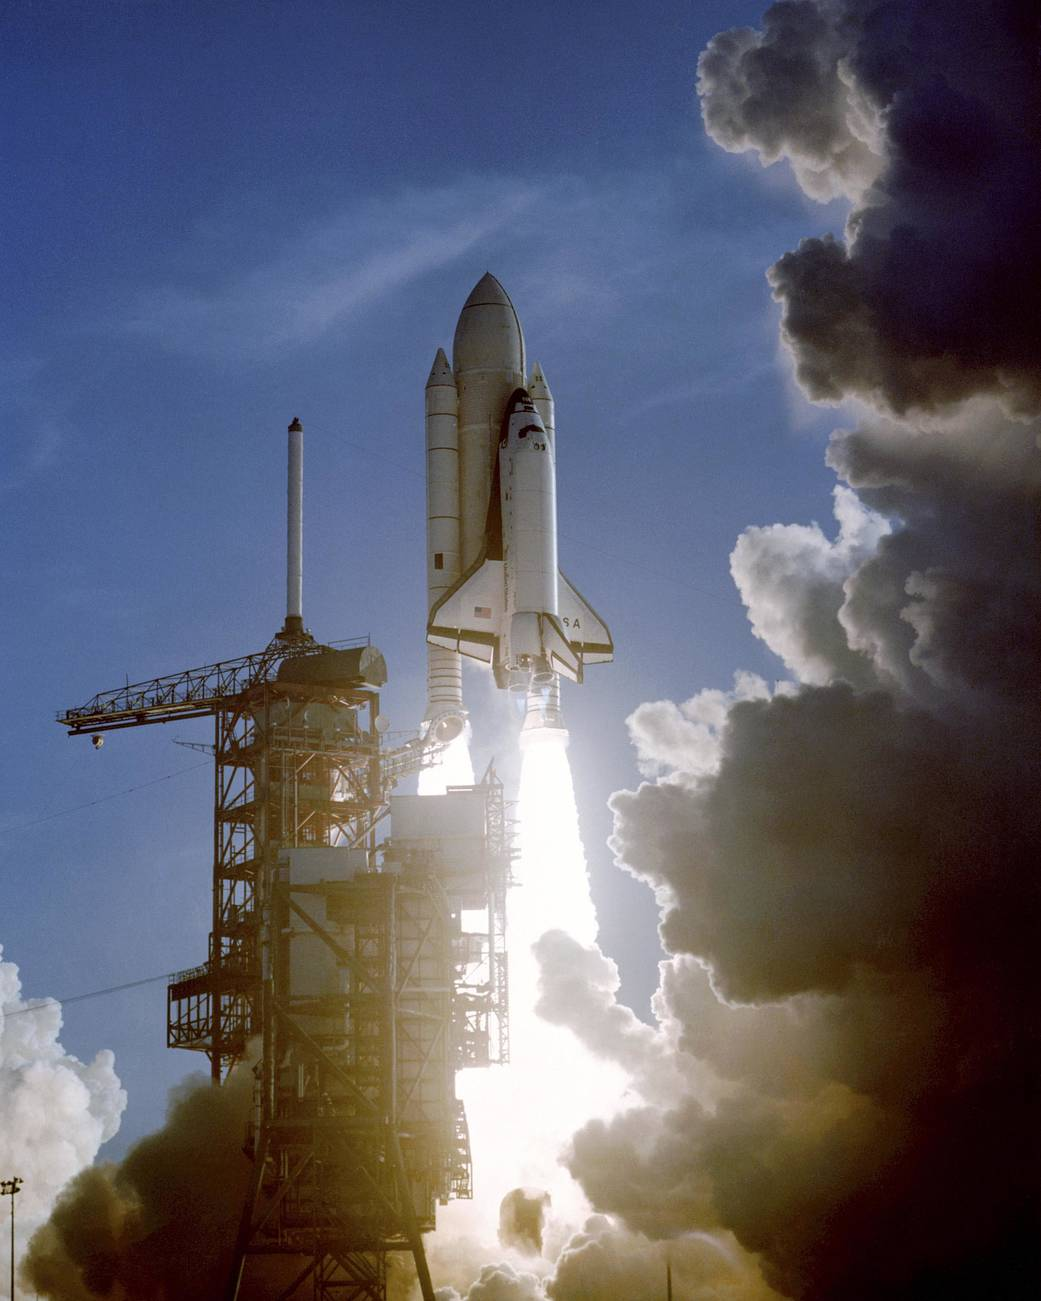
\includegraphics[height=\paperheight]{cover-nasa.jpg}};
\fill[white,opacity=.91] (0,0) rectangle (595.276,89.5);
\fill[studiumInk,opacity=.96] (0,585.5) rectangle (595.276,841.89);
\node[anchor=west,text=studiumInk,font=\sffamily\bfseries\fontsize{18}{20}\selectfont,inner sep=0pt] at (51.223,38.5){STUDIUM};
\fill[studiumCyan] (51.223,61.5) rectangle (80.8,63.7);
\node[anchor=west,text=studiumInk,font=\sffamily\fontsize{9}{11}\selectfont,inner sep=0pt] at (89.49,65.5){BIBLIOTECA DE INGENIERÍA};
\node[anchor=west,text=studiumCyan,font=\sffamily\bfseries\fontsize{10}{12}\selectfont,inner sep=0pt] at (51.223,608){MANUAL UNIVERSITARIO};
\node[anchor=north west,text=white,text width=493pt,font=\rmfamily\bfseries\fontsize{33}{36}\selectfont,inner sep=0pt] at (51.223,636){#1};
\node[anchor=west,text=white!82!studiumInk,font=\sffamily\fontsize{11}{14}\selectfont,inner sep=0pt] at (51.223,732){#2};
\node[anchor=west,text=white,font=\sffamily\bfseries\fontsize{10}{12}\selectfont,inner sep=0pt] at (51.223,758){GRADO EN INGENIERÍA AEROESPACIAL};
\node[anchor=west,text=white!82!studiumInk,font=\sffamily\fontsize{10}{12}\selectfont,inner sep=0pt] at (51.223,773){Universidad de León};
\draw[white!75!studiumInk,line width=.4pt] (51.223,786) -- (544.05,786);
\node[anchor=west,text=white!82!studiumInk,font=\sffamily\fontsize{10}{12}\selectfont,inner sep=0pt] at (51.223,810){2026};
\node[anchor=east,text=white,font=\sffamily\bfseries\fontsize{10}{12}\selectfont,inner sep=0pt] at (544.05,810){I Edición};
\end{scope}\end{tikzpicture}\null\end{titlepage}\hypersetup{pageanchor=true}}

\hypersetup{pdftitle={Tecnología Aeroespacial — Simulacros originales}}
\begin{document}
\portada{SIMULACROS\\ORIGINALES}{Tecnología Aeroespacial}
\frontmatter
\chapter*{Instrucciones}
Este cuaderno contiene tres simulacros originales con tiempos y reparto de puntos orientativos. No reproduce exámenes anteriores ni representa una propuesta oficial de evaluación de la ULE. Los enunciados incluyen los datos necesarios. Las soluciones se encuentran en el cuaderno de problemas, no en este documento.

Presente datos, incógnitas, hipótesis, modelo físico, desarrollo simbólico, sustitución, unidades, interpretación, comprobación y limitaciones. Si un estado resulta imposible bajo el modelo, explique el criterio que lo detecta en lugar de forzar una raíz o eliminar un signo. La corrección debe valorar el razonamiento además del número final. Datos comunes: $T_0=288.15\,\mathrm K$, $p_0=101325\,\mathrm{Pa}$, $g_0=9.80665\,\mathrm{m/s^2}$, $R_a=287.05287\,\mathrm{J/(kg\,K)}$, $\gamma=1.4$ y gradiente troposférico $-0.0065\,\mathrm{K/m}$.
\tableofcontents
\mainmatter
\chapter{Simulacro 1: atmósfera, medidas y fluidos}
\caja{Condiciones editoriales}{Tiempo sugerido: 110 minutos. Puntuación: 10 puntos. Se permite una calculadora y el formulario adjunto. Esta propuesta no describe las condiciones oficiales de examen. Todas las altitudes ISA son geopotenciales. Use $g_0=9.80665\,\mathrm{m/s^2}$, $R_a=287.05287\,\mathrm{J/(kg\,K)}$, $\gamma=1.4$.}
\section{Cuestiones razonadas: 2 puntos}
Explique la diferencia entre altitud de presión y altitud de densidad, indicando qué efecto produce un día cálido a presión fija. Distinga presión dinámica y presión de impacto y justifique cuándo pueden igualarse aproximadamente. Defina línea de corriente y trayectoria, indicando una condición suficiente para que coincidan. Reparta la respuesta en tres explicaciones breves con sus hipótesis.
\section{Globo en atmósfera estándar: 3 puntos}
Un globo de helio se encuentra a $H=3500\,\mathrm m$. Su volumen es $450\,\mathrm{m^3}$ y la masa de envolvente y equipos es $100\,\mathrm{kg}$. El helio tiene la misma presión y temperatura que el ambiente; su constante de gas es $2077.1\,\mathrm{J/(kg\,K)}$. La envolvente admite ese volumen sin sobrepresión apreciable.
\begin{enumerate}[label=\alph*)]
\item Determine $T,p,\rho_a$ del aire y la densidad del helio. (1.2)
\item Obtenga la masa máxima de carga útil para equilibrio vertical, contabilizando el gas. (1.0)
\item Escriba el balance de fuerzas con una carga cinco kilogramos menor. Interprete el signo de la fuerza neta y explique qué dato faltaría para calcular una velocidad de ascenso estacionaria. (0.8)
\end{enumerate}
\section{Pitot subsónico: 3 puntos}
Una aeronave vuela en ISA a $H=5500\,\mathrm m$. La toma frontal mide $p_t=53800\,\mathrm{Pa}$ y la toma estática es ideal. Se supone flujo subsónico, gas perfecto y desaceleración isentrópica hasta la toma.
\begin{enumerate}[label=\alph*)]
\item Calcule $p$, $T$ y $\rho$ del ambiente. (0.7)
\item Determine Mach y TAS a partir de la relación compresible. Compruebe el régimen supuesto. (1.3)
\item Calcule la TAS que resultaría de igualar $p_t-p$ a $\rho V^2/2$, y cuantifique su error relativo frente a la inversión anterior. (1.0)
\end{enumerate}
\section{Qué permite saber continuidad: 2 puntos}
Un conducto estacionario recibe aire con $\rho_1=1.15\,\mathrm{kg/m^3}$, $A_1=0.50\,\mathrm{m^2}$ y $V_1=80\,\mathrm{m/s}$. A la salida se conocen $\rho_2=1.05\,\mathrm{kg/m^3}$ y $A_2=0.35\,\mathrm{m^2}$. No hay fugas.
\begin{enumerate}[label=\alph*)]
\item Halle el caudal másico y la velocidad de salida. (1.0)
\item Indique si puede conservarse $AV$ y si estos datos permiten conocer de forma única la presión de salida. Identifique información o hipótesis adicionales necesarias. (1.0)
\end{enumerate}
\chapter{Simulacro 2: geometría, polar y crucero}
\caja{Condiciones editoriales}{Tiempo sugerido: 120 minutos. Puntuación: 10 puntos. Todas las relaciones aerodinámicas de este simulacro son modelos educativos válidos en la región adherida y de Mach bajo que se debe comprobar. La altitud es geopotencial.}
\section{Definición del vehículo}
Una aeronave de peso instantáneo $W=34000\,\mathrm N$ posee un ala trapezoidal de $b=12.0\,\mathrm m$, cuerda de raíz $c_r=2.10\,\mathrm m$ y estrechamiento $\lambda=0.50$. El perfil tiene pendiente $a_0=6.0\,\mathrm{rad^{-1}}$ y ángulo de sustentación nula $\alpha_0=-2.0^\circ$. Adopte teoría lineal de ala finita con $e_i=0.91$. La polar del vehículo es
\[
C_D=0.026+\left[\frac{1}{\pi e_iAR}+0.007\right]C_L^2.
\]
Para este problema se iguala la sustentación del ala a la de la aeronave y se omiten las contribuciones de fuselaje y cola a la pendiente. El vehículo vuela a $H=2500\,\mathrm m$ en ISA, rectilíneo y horizontal, a TAS de $72\,\mathrm{m/s}$. Se da $C_{L\max}=1.45$ y empuje horizontal.
\section{Geometría y significado de los parámetros: 2 puntos}
Obtenga $S$, $AR$, $K$ total y $e_O$. Explique por qué $e_O$ y $e_i$ no coinciden en este modelo. Determine qué parte de $C_D-C_{D0}$ es inducida y qué parte es resistencia de perfil dependiente de sustentación, sin atribuir ambas al mismo fenómeno.
\section{Condición de crucero: 3 puntos}
Calcule la densidad ISA, el $C_L$ requerido, la pendiente tridimensional, el ángulo de ataque en grados, el coeficiente de resistencia, el empuje necesario y la potencia aerodinámica necesaria. Compruebe el margen respecto de $C_{L\max}$ y el número de Mach aproximado. Explique la diferencia entre la potencia calculada y la potencia que debería entregar un eje de hélice.
\section{Óptimo y pérdida de empuje: 3 puntos}
Derive la condición de mínima resistencia y calcule $D_{\min}$ y su TAS. El empuje máximo disponible se reduce ahora al 80\,\% del que exigía el crucero anterior y se considera constante con velocidad en el intervalo. Determine si existe cualquier velocidad que mantenga vuelo nivelado con el mismo peso, altitud y polar. Justifique por mínimo global y por discriminante, evitando suponer que la respuesta se obtiene reduciendo la velocidad un 20\,\%.
\section{Teoría aplicada: 2 puntos}
Si se aumenta el ángulo de ataque conservando peso y altitud, razone qué debe cambiar para seguir en equilibrio. Después considere un empuje constante de $1.2D_{\min}$: plantee las dos raíces matemáticas de velocidad e indique cómo se decide cuáles son físicamente admisibles. No hace falta atribuir estabilidad dinámica a ninguna raíz.
\chapter{Simulacro 3: actuaciones, espacio e integración}
\caja{Condiciones editoriales}{Tiempo sugerido: 120 minutos. Puntuación: 10 puntos. Datos educativos; no representan una aeronave ni misión certificadas. Justifique cada simplificación y utilice unidades SI.}
\section{Ascenso y giro: 4 puntos}
Una aeronave de $W=36000\,\mathrm N$ y $S=20\,\mathrm{m^2}$ opera en aire de $\rho=0.90\,\mathrm{kg/m^3}$ a TAS $65\,\mathrm{m/s}$. La polar es $C_D=0.024+0.055C_L^2$, el empuje máximo $4300\,\mathrm N$ y $C_{L\max}=1.45$.
\begin{enumerate}[label=\alph*)]
\item Calcule la resistencia nivelada y una estimación de la velocidad de ascenso usando la resistencia nivelada como aproximación de primer orden. Declare esa aproximación. (1.3)
\item Para un giro horizontal coordinado de $45^\circ$, determine factor de carga, $C_L$ requerido y resistencia a la misma velocidad. (1.3)
\item Compruebe por separado sustentación máxima y empuje disponible. Determine si el giro se sostiene a esa velocidad y explique por qué un margen frente a pérdida no basta para afirmarlo. (1.4)
\end{enumerate}
\section{Etapa cohete y órbita: 3 puntos}
Una etapa tiene $m_0=1800\,\mathrm{kg}$, $m_f=650\,\mathrm{kg}$ e $I_{sp}=298\,\mathrm s$ constante. Calcule su $\Delta V$ ideal. Una órbita circular terrestre de radio $6971\,\mathrm{km}$ se modela con $\mu_g=3.986004418\times10^{14}\,\mathrm{m^3/s^2}$. Halle velocidad y periodo orbitales. Explique por qué comparar ambos valores de velocidad no constituye un dimensionamiento completo de lanzamiento desde la superficie, aunque sea un primer contraste de escala.
\section{Energía de sistemas: 3 puntos}
Un circuito hidráulico suministra $Q=3.0\times10^{-4}\,\mathrm{m^3/s}$ con incremento de presión de $14\,\mathrm{MPa}$ y rendimiento global $0.80$. Obtenga la potencia de entrada. De forma independiente, una carga eléctrica ideal demanda $1200\,\mathrm W$ a $28\,\mathrm V$, con resistencia total de ida y retorno de $0.040\,\Omega$.
\begin{enumerate}[label=\alph*)]
\item Halle corriente nominal y pérdida resistiva utilizando esa corriente. Indique la aproximación en el uso de 28 V como tensión de la carga. (1.0)
\item Compare potencias y describa un camino de disipación térmica que el diseño debería prever. (1.0)
\item Si se duplican dos bombas pero ambas dependen de una única barra eléctrica, identifique una causa común que pueda perder la función. Distinga redundancia de independencia. (1.0)
\end{enumerate}

\chapter{Simulacro 4: compresibilidad, ondas de choque y perfiles}
\caja{Condiciones editoriales}{Tiempo sugerido: 110 minutos. Puntuación: 10 puntos. Se permite una calculadora. Esta propuesta no describe las condiciones oficiales de examen. Use ISA con altitud geopotencial, $g_0=9.80665\,\mathrm{m/s^2}$, $R_a=287.05287\,\mathrm{J/(kg\,K)}$ y $\gamma=1.4$.}
\section{Cuestiones razonadas: 2 puntos}
Explique por qué a través de un choque normal estacionario aumenta la entropía y disminuye la presión total mientras la temperatura total se conserva. Distinga el ángulo de Mach del ángulo de un choque oblicuo e indique cuándo coinciden. Justifique por qué la corrección de Prandtl-Glauert no sirve en régimen supersónico ni en las cercanías de $M=1$. Reparta la respuesta en tres explicaciones breves con sus hipótesis. (0.7 + 0.7 + 0.6)
\section{Pitot en vuelo supersónico: 3 puntos}
Una aeronave de investigación vuela en ISA a $H=12000\,\mathrm m$ con $M=2.0$. Se supone gas perfecto, un choque normal desprendido frente a la toma de un tubo Pitot y desaceleración isentrópica posterior hasta la toma.
\begin{enumerate}[label=\alph*)]
\item Calcule $p$, $T$, $\rho$, la velocidad del sonido y la velocidad de vuelo. (0.8)
\item Obtenga el Mach tras el choque y los cocientes de presión, densidad y temperatura estáticas a través de él, además de $p_{t2}/p_{t1}$. (1.2)
\item Calcule la presión de remanso $p_{t2}$ que mediría el Pitot. Si un observador aplicase por error la fórmula subsónica a $p_{t2}$ y $p$, ¿qué Mach leería? Interprete la diferencia. (1.0)
\end{enumerate}
\section{Cuña y choque oblicuo: 3 puntos}
Una corriente de aire con $M_1=2.5$ incide sobre una cuña que produce un choque oblicuo unido de ángulo $\beta=40^\circ$.
\begin{enumerate}[label=\alph*)]
\item Determine el ángulo de desviación $\theta$ de la cuña mediante la relación $\theta$-$\beta$-$M$. (1.0)
\item Calcule los cocientes de presión, densidad y temperatura estáticas a través del choque. (1.0)
\item Obtenga el Mach tras el choque, compruebe que sigue siendo supersónico y explique por qué no existe solución con choque unido si $\theta$ supera un máximo que depende de $M_1$. (1.0)
\end{enumerate}
\section{Perfil y compresibilidad: 2 puntos}
Un perfil de cuerda $c=1.8\,\mathrm m$ vuela a $H=3000\,\mathrm m$ en ISA con $M=0.6$. Use teoría de perfil delgado con pendiente $2\pi\,\mathrm{rad^{-1}}$, $\alpha=4^\circ$ y $\alpha_{L0}=-1.5^\circ$. La viscosidad sigue la ley de Sutherland: $\mu=1.716\times10^{-5}(T/273.15)^{3/2}(273.15+110.4)/(T+110.4)$.
\begin{enumerate}[label=\alph*)]
\item Calcule velocidad de vuelo, densidad y número de Reynolds. (1.0)
\item Obtenga $C_l$ incompresible y con corrección de Prandtl-Glauert; comente su validez. (1.0)
\end{enumerate}

\chapter{Simulacro 5: motores de explosión, de reacción y cohete}
\caja{Condiciones editoriales}{Tiempo sugerido: 120 minutos. Puntuación: 10 puntos. Se permite una calculadora. Esta propuesta no describe las condiciones oficiales de examen. Salvo indicación, use $\gamma=1.4$ y $R_a=287.05287\,\mathrm{J/(kg\,K)}$ con calores específicos constantes. $g_0=9.80665\,\mathrm{m/s^2}$.}
\section{Cuestiones razonadas: 2 puntos}
Explique por qué el rendimiento térmico del ciclo Otto ideal depende solo de la relación de compresión y por qué no puede aumentarse indefinidamente en un motor real. Justifique por qué un turborreactor tiene mayor rendimiento propulsivo cuanto más se acerca la velocidad de salida a la de vuelo y qué se pierde a cambio. Defina impulso específico e indique por qué el valor en vacío es mayor que a nivel del mar para una misma tobera. (0.7 + 0.7 + 0.6)
\section{Ciclo Otto ideal: 2.5 puntos}
Un motor de encendido por chispa admite aire a $T_1=300\,\mathrm K$ y $p_1=95\,\mathrm{kPa}$, con relación de compresión $r=9$. El aporte de calor a volumen constante es $q=1.2\,\mathrm{MJ/kg}$.
\begin{enumerate}[label=\alph*)]
\item Calcule temperatura y presión al final de la compresión isentrópica. (0.8)
\item Calcule temperatura y presión tras el aporte de calor y la temperatura al final de la expansión. (0.9)
\item Determine el rendimiento térmico, el trabajo neto específico y compruebe el balance de calor cedido de dos formas. (0.8)
\end{enumerate}
\section{Turborreactor con tobera adaptada: 2.5 puntos}
Un turborreactor ingiere $45\,\mathrm{kg/s}$ de aire en vuelo a $220\,\mathrm{m/s}$. El dosado másico es $f=0.015$ y los gases salen a $620\,\mathrm{m/s}$ con la presión ambiente.
\begin{enumerate}[label=\alph*)]
\item Calcule el empuje. (1.0)
\item Obtenga la potencia propulsiva, el incremento de energía cinética de la corriente y el rendimiento propulsivo. (1.0)
\item Calcule el consumo específico de empuje en $\mathrm{kg/(N\,s)}$ y en $\mathrm{kg/(N\,h)}$. (0.5)
\end{enumerate}
\section{Tobera de un motor cohete: 3 puntos}
La cámara de un motor cohete está a $p_c=5\,\mathrm{MPa}$ y $T_c=3400\,\mathrm K$. Los gases tienen $\gamma=1.2$ y $R=380\,\mathrm{J/(kg\,K)}$. La garganta tiene $A_t=0.04\,\mathrm{m^2}$ y la tobera se diseña para $p_e=60\,\mathrm{kPa}$. Flujo isentrópico unidimensional.
\begin{enumerate}[label=\alph*)]
\item Calcule el gasto másico, la temperatura y la velocidad de salida. (1.0)
\item Obtenga el área de salida, la relación de expansión y el Mach de salida. (1.0)
\item Calcule el empuje al nivel del mar ($p_a=101325\,\mathrm{Pa}$) y en vacío, y los impulsos específicos correspondientes. Indique el régimen de funcionamiento de la tobera al nivel del mar. (1.0)
\end{enumerate}

\chapter{Simulacro 6: estructuras, materiales y cargas de vuelo}
\caja{Condiciones editoriales}{Tiempo sugerido: 120 minutos. Puntuación: 10 puntos. Se permite una calculadora. Esta propuesta no describe las condiciones oficiales de examen. Los datos de material son docentes: $E=70\,\mathrm{GPa}$ y límite elástico $\sigma_y=300\,\mathrm{MPa}$. Use ISA, $g_0=9.80665\,\mathrm{m/s^2}$ y $R_a=287.05287\,\mathrm{J/(kg\,K)}$.}
\section{Cuestiones razonadas: 2 puntos}
Explique por qué en un recipiente cilíndrico de pared delgada la tensión circunferencial es el doble que la longitudinal. Indique cuándo es válida la fórmula de Euler para una columna y qué ocurre con la carga crítica si se duplica la longitud o se empotran ambos extremos. Defina la velocidad de maniobra y explique qué protege. (0.7 + 0.7 + 0.6)
\section{Fuselaje presurizado: 3 puntos}
Un fuselaje cilíndrico de radio $r=1.9\,\mathrm m$ y espesor $t=1.6\,\mathrm{mm}$ mantiene una altitud de cabina de $2400\,\mathrm m$ mientras la aeronave cruza a $11000\,\mathrm m$ (ISA para ambas).
\begin{enumerate}[label=\alph*)]
\item Calcule las presiones de cabina y exterior y su diferencia. (0.8)
\item Obtenga las tensiones circunferencial y longitudinal, la tensión equivalente de von Mises y el coeficiente de seguridad estático. (1.2)
\item Explique por qué ese coeficiente no garantiza la vida a fatiga ni la tolerancia al daño. (1.0)
\end{enumerate}
\section{Pandeo de una barra tubular: 2.5 puntos}
Una barra tubular biarticulada de diámetro exterior $40\,\mathrm{mm}$, interior $36\,\mathrm{mm}$ y longitud $1.2\,\mathrm m$ trabaja a compresión.
\begin{enumerate}[label=\alph*)]
\item Calcule momento de inercia, área y carga crítica de Euler. (1.0)
\item Obtenga la esbeltez, compruebe la validez de Euler con la esbeltez límite $\pi\sqrt{E/\sigma_y}$ y determine si gobierna el pandeo o la fluencia. (1.0)
\item Indique cómo cambia la carga crítica con empotramiento doble. (0.5)
\end{enumerate}
\section{Maniobra y ráfaga: 2.5 puntos}
Una aeronave ligera de $W=11800\,\mathrm N$ y $S=16\,\mathrm{m^2}$ tiene $C_{L\max}=1.5$. Se toma $\rho_0=1.225\,\mathrm{kg/m^3}$ y un factor de carga límite $n_{\max}=3.8$.
\begin{enumerate}[label=\alph*)]
\item Calcule la velocidad de pérdida con $n=1$ y la velocidad de maniobra. (1.0)
\item Para una ráfaga discreta de $7.6\,\mathrm{m/s}$ a una velocidad equivalente de $45\,\mathrm{m/s}$ y pendiente de sustentación $5.0\,\mathrm{rad^{-1}}$, calcule el incremento y el factor de carga resultante, sin factor de atenuación. (1.0)
\item Compare con el límite e indique dos simplificaciones del modelo. (0.5)
\end{enumerate}

\chapter{Simulacro 7: navegación, ortodrómica y actuaciones de pista}
\caja{Condiciones editoriales}{Tiempo sugerido: 110 minutos. Puntuación: 10 puntos. Se permite una calculadora. Esta propuesta no describe las condiciones oficiales de examen. Tierra esférica de radio $6371\,\mathrm{km}$; ISA con altitud geopotencial, $g_0=9.80665\,\mathrm{m/s^2}$, $R_a=287.05287\,\mathrm{J/(kg\,K)}$.}
\section{Cuestiones razonadas: 2 puntos}
Distinga velocidad verdadera, velocidad respecto al suelo y velocidad indicada. Explique por qué una ruta ortodrómica no mantiene un rumbo constante y cuándo conviene la loxodrómica. Justifique por qué un aeródromo elevado en un día cálido alarga el recorrido de despegue. (0.7 + 0.7 + 0.6)
\section{Triángulo de vientos: 3 puntos}
Una aeronave de $\mathrm{TAS}=75\,\mathrm{m/s}$ debe seguir una derrota $090^\circ$. El viento sopla de $030^\circ$ con $15\,\mathrm{m/s}$.
\begin{enumerate}[label=\alph*)]
\item Calcule las componentes longitudinal y transversal del viento respecto a la derrota. (0.8)
\item Determine el ángulo de corrección de deriva, el rumbo a volar y la velocidad respecto al suelo. (1.4)
\item Calcule el tiempo de un tramo de $180\,\mathrm{km}$. (0.8)
\end{enumerate}
\section{Distancia y rumbo inicial ortodrómicos: 2.5 puntos}
Entre dos aeropuertos de coordenadas redondeadas $40.47^\circ\mathrm N,\,3.56^\circ\mathrm W$ y $41.30^\circ\mathrm N,\,2.08^\circ\mathrm E$.
\begin{enumerate}[label=\alph*)]
\item Calcule el ángulo central por la fórmula haversine y la distancia ortodrómica. (1.5)
\item Obtenga el rumbo inicial y explique su variación a lo largo de la ruta. (1.0)
\end{enumerate}
\section{Recorrido de despegue: 2.5 puntos}
Una aeronave ligera de $W=15000\,\mathrm N$, $S=16\,\mathrm{m^2}$ y $C_{L\max}=1.6$ despega con empuje estático constante $3200\,\mathrm N$ al nivel del mar ($\rho_0=1.225\,\mathrm{kg/m^3}$), con coeficiente de rodadura $\mu=0.03$. Se modela una aceleración media constante $a=g_0(T/W-\mu)$, sin resistencia aerodinámica, y la velocidad de despegue es $1.2V_s$.
\begin{enumerate}[label=\alph*)]
\item Calcule el recorrido al nivel del mar. (0.8)
\item Repítalo en un aeródromo a $2000\,\mathrm m$ ISA con temperatura ISA$+20\,\mathrm K$, suponiendo que el empuje es proporcional a la densidad. (1.2)
\item Compare ambos resultados e indique tres efectos que el modelo omite. (0.5)
\end{enumerate}

\chapter{Simulacro 8: sistemas hidráulicos, eléctricos y alcance}
\caja{Condiciones editoriales}{Tiempo sugerido: 110 minutos. Puntuación: 10 puntos. Se permite una calculadora. Esta propuesta no describe las condiciones oficiales de examen. Datos educativos; no representan una aeronave ni un componente certificados. $g_0=9.80665\,\mathrm{m/s^2}$.}
\section{Cuestiones razonadas: 2 puntos}
Explique por qué un actuador hidráulico de doble efecto con vástago de un solo lado desarrolla menos fuerza y más velocidad en retracción que en extensión. Distinga la capacidad nominal de una batería de la energía realmente utilizable. Justifique por qué la ecuación de Breguet supone cociente $L/D$ y consumo específico constantes y qué ocurre si no lo son. (0.7 + 0.7 + 0.6)
\section{Actuador hidráulico: 3 puntos}
Un actuador de doble efecto tiene pistón de $50\,\mathrm{mm}$ de diámetro y vástago de $25\,\mathrm{mm}$. El sistema trabaja a $21\,\mathrm{MPa}$ y el caudal disponible es $1.0\times10^{-3}\,\mathrm{m^3/s}$.
\begin{enumerate}[label=\alph*)]
\item Calcule la fuerza máxima en extensión y en retracción. (0.8)
\item Calcule las velocidades de extensión y de retracción con ese caudal. (0.7)
\item Con una carga de $30\,\mathrm{kN}$ en extensión, calcule potencia hidráulica, potencia útil y potencia disipada; la potencia de entrada de una bomba de rendimiento $0.85$; y la tasa de calentamiento si $18\,\mathrm{kg}$ de fluido ($c=1900\,\mathrm{J/(kg\,K)}$) absorben el calor sin enfriamiento. (1.5)
\end{enumerate}
\section{Batería y cableado: 2.5 puntos}
Una batería de $24\,\mathrm V$ y $40\,\mathrm{Ah}$ alimenta una carga de $15\,\mathrm A$ continuos mediante un cable de cobre ($\rho_{Cu}=1.72\times10^{-8}\,\Omega\,\mathrm m$) de $6\,\mathrm{mm^2}$ y $12\,\mathrm m$ de longitud total de ida y vuelta.
\begin{enumerate}[label=\alph*)]
\item Calcule la autonomía si solo es utilizable el $80\,\%$ de la capacidad. (0.8)
\item Calcule la resistencia del cable, la caída de tensión y la pérdida por efecto Joule. (1.2)
\item Indique la tensión en la carga y la caída relativa. (0.5)
\end{enumerate}
\section{Alcance y autonomía de Breguet: 2.5 puntos}
Una aeronave a reacción vuela a $230\,\mathrm{m/s}$ con $L/D=16$ y consumo específico $1.7\times10^{-5}\,\mathrm{kg/(N\,s)}$. La razón entre pesos inicial y final es $1.25$.
\begin{enumerate}[label=\alph*)]
\item Calcule el alcance de Breguet. (1.2)
\item Calcule la autonomía. (0.8)
\item Obtenga la fracción de combustible respecto al peso inicial e indique dos condiciones que la ecuación supone. (0.5)
\end{enumerate}


\end{document}
